\documentclass[a4paper,12pt,titlepage]{report}

\usepackage{amsmath}
\usepackage{fullpage}
\usepackage{tikz}

\title{Improving the Interconnection Network of a Brain Simulator}
\author{Jonathan Heathcote}
\date{The University of Manchester}

% Number subsubsections
\setcounter{secnumdepth}{3}

\begin{document}
	
	\maketitle
	
	\begin{abstract}
		
		The human brain is one of the most complex structures known to man and
		allows us to perform remarkable range of computational feats completely
		inaccessible to any machine. Recent efforts to study the brain have led
		researchers to devise novel massively-parallel computer architectures in
		order to cope with the unique demands of brain simulation software. The
		SpiNNaker project is developing one such machine based on over 1,000,000
		custom low-power ARM processors. My research aims to improve the way in
		which these processors connect together to improve the performance of
		simulations and other software on the system.
		
	\end{abstract}
	
	\tableofcontents
	
	\listoffigures
	
	\listoftables
	
	\chapter{Introduction}
	
	% %Some high-level motivation and context to sort of set the scene before going
	% %into what other folk have done and what I'm hoping to do.
	% 
	% Modern computer systems represent some of the most complex devices ever
	% constructed. Indeed, current computer technologies have enabled everything
	% from global, instantaneous communications via the internet to faster and more
	% effective cancer treatments\cite{nassif}. Despite this, the brain still
	% outperforms conventional digital computers at many tasks.
	% 
	% Considerable effort has been made by researchers to understand how the brain
	% works. The small-scale operation of individual neurons in the brain is now
	% relatively well understood but the manner of their interactions is still not
	% clear. Current efforts to understand the brain attempt to model it as a
	% biological computer. Such biological computers differ greatly from digital
	% computers and so simulating their behaviour using existing technology is
	% challenging.
	% 
	% Recent neural models such as the Spaun brain simulator \cite{eliasmith12}
	% exhibit a remarkable range of cognitive abilities such as memory, problem
	% solving and pattern recognition. As well as realistic functional behaviour,
	% they also respond to failures, such as neuron death, just as real brains do
	% exhibiting a gradual decline in functionality. The existence of realistic
	% models means studying the properties of the brain in a highly controlled,
	% observable manner as in a simulator is becoming a possibility.
	
	Modern computer systems represent some of the most complex devices ever
	constructed. Indeed, current computer technologies have enabled everything
	from global, instantaneous communications via the internet to faster and more
	effective cancer treatments\cite{nassif}. Despite this, the brain still
	outperforms conventional digital computers at many tasks.
	
	Considerable effort has been made by researchers to understand how the brain
	works. The small-scale operation of individual neurons in the brain is now
	relatively well understood but the manner of their interactions is still not
	clear. By modelling the behaviour of networks of neurons it is possible to
	gain a better understanding of their collective behaviour. Such models are
	challenging to fit into modern computer architectures since the vast
	parallelism available to individual neurons in a brain is in sharp contrast
	with the computing resources available today.

	In this introduction I hope to elaborate on the role that modelling has on
	understanding the brain and on the work being done to build machines to fulfil
	this task. I also outline the specific aspect of these machines on which my
	work will focus, the interconnection network, and its importance in achieving
	the wider goal.
	
	\section{Why Model The Brain?}
	
		
		%% TODO REWORD BELOW
		
		Cutting-edge neural models, such as Spaun \cite{eliasmith12}, are able to
		demonstrate a remarkable range of cognitive abilities such as memory,
		problem solving and pattern recognition. Notably, Spaun exhibits very
		similar behaviour to humans in terms of the way its memory degrades over
		time. It also suffers the same gradual reduction in function as random
		neurons die off. This level of realism means that experiments which would
		not be possible may become feasible using the Spaun model.
		
		In addition to Spaun, many other neural models have emerged. In distinct
		contrast to Spaun, researchers on the Blue Brain project \cite{markram06}
		have focused on developing high-accuracy simulations of much smaller
		collections of neurons. Such models are highly biologically plausible but
		do not result in the complex, high-level behaviour shown by simulators such
		as Spaun.
		
		Unfortunately these models present a great challenge to modern computer
		systems. The Spaun simulator takes around two and a half hours of compute
		time to simulate one second of neural activity on a high-end workstation
		computer. The Blue Brain project requires a commercial super-computer to
		reach simulation speeds still around an order of magnitude slower than
		biological real-time. The basic mechanism of these neural simulators, and
		their computational challenges is described in further detail in
		\S\ref{sec:simulating-brains}.
	
	\section{Conventional Approaches}
	
		% Why not use a big ass-computer? Well big computers are good for computation
		% but neural stuff is all about communication. Not so great. As mentioned
		% there is another way 
		
		Conventional super computers are designed to provide immense computational
		power performing quadrillions ($10^{15}$) of calculations to be performed
		per second. Despite these extremely impressive feats of computation, these
		machines often feature substantially less impressive interconnection
		networks tying them together. This balance of computation and communication
		is contrary to the brain whose neurons represent relatively little
		computational power but are extraordinarily well connected.
		
		The Blue Brain project is notable in its use of conventional super
		computers. Though they are severely limited in the size of their models,
		only around 100,000 neurons compared with almost 100 billion in the human
		brain, they are able to precisely simulate the detailed biological and
		chemical processes occurring within each neuron.
		
		\S\ref{sec:super-computers} goes into greater detail on current super
		computer architectures and their strengths and weaknesses.
	
	\section{Why Interconnect Matters}
		
		My research focuses on the challenge of developing architectures designed
		for the simulation of large-scale networks, such as Spaun, which are heavily
		communication bound.
		
		The SpiNNaker project \cite{furber06} has developed a novel computer
		architecture which emphasises communication over computation based on a
		network of over one million small, low-power processors. The purpose built
		interconnection network is designed to handle neural simulations of up to
		one billion neurons running in biological real-time. A detailed introduction
		to the SpiNNaker architecture is given in \S\ref{sec:spinnaker}.
		
		SpiNNaker's interconnection network is designed to allow efficient
		communication of signals produced by the simulated neurons which typically
		only need to travel short distances in the system. As the system scales, new
		types of interconnection network have been introduced in order to keep the
		wiring in the system practical. \S\ref{sec:high-speed-serial} describes the
		technology used to simplify the system's wiring. Preliminary work, described
		in \S\ref{sec:interconnect-modelling}, has been conducted to asses the
		impact of these changes for neural network simulation. It shows the impact
		changes in the system's interconnect can have on the time taken by neural
		signals to move through the system.
		
		The topic of practical issues when designing interconnect issues is studied
		in \S\ref{sec:wiring-up-large-spinnaker-machines} where the task of wiring
		up large SpiNNaker systems consisting of 1,200 of connected circuit boards
		is tackled. This is followed up by the development of an unconventional
		semi-random interconnection network which takes into account these wiring
		considerations in \S\ref{sec:small-world-super-computers}. This design of
		network has the potential to improve the performance of SpiNNaker's
		architecture with a minimal cost in increased cabling requirements.
	
		% SpiNNaker is a neural simulator emphasising communication over computation
		% by using lots of low-powered cores. It hopes to do real-time simulation. It
		% uses a very straight-forward mesh interconnect which suffers very long
		% latencies for non-local traffic. Alternative topologies can overcome this.
	
		My work hopes to develop a new architecture with a focus on the
		interconnection network, a key aspect of a machine targeted at communication
		bound problems such as neural simulation. Section \S\ref{sec:research-plan}
		outlines the plan of research I intend to take to reach this goal following
		on from my preliminary studies.

	\chapter{Background}
	\label{chap:background}
	
	This chapter gives an overview of the work being done on brain simulators. It
	begins with a history of the models used to simulate the brain which lead to
	the current generation of `spiking neural networks' and the computational
	challenges these bring. The latest super-computer technology is then presented
	with an explanation of its unsuitability for neural simulation. This is
	followed by a discussion of the various attempts made to produce a
	special-purpose architecture for this task looking in particular at the highly
	flexible SpiNNaker architecture. The chapter concludes by examining the
	technology used in SpiNNaker and other super-computers to allow fast
	communication within these systems.
	
	\section{Simulating Brains}
		
		\label{sec:simulating-brains}
		
		% Background on brain simulation techniques.
		
		Efforts to simulate the brain focus on building approximate but
		representative models of the brain's behaviour. Most current brain models
		attempt to capture the way that neurons in the brain behave and communicate
		with each other. Typically, the network is expressed as a graph of neurons
		which take inputs from other neurons and perform some simple computation to
		produce an output which is, in turn, connected to other neurons. This type
		of model is known generally as an artificial neural network (ANN).
		
		\subsection{Generations of ANN}
			
			The development of ANNs can be divided up into three coarse generations,
			each increasing their level of biological realism \cite{vainbrand11}.
			
			The first generation of ANNs, such as the McCulloch-Pitts threshold neuron
			\cite{mcculloch43}, consisted of testing if a simple, linear function of
			the neuron's inputs was above a threshold value and outputting either a
			`high' or `low' signal. The function used in each neuron along with the
			pattern of connectivity in the network define the behaviour of the network
			as a whole.
			
			It was realised that communication between neurons was not level-based but
			instead appeared to be based on the rate at which electrical `spikes' are
			fired by neurons to their neighbours. The second generation of ANNs seek
			to model this by representing the `firing rate' as their output in a
			continuous value \cite{maass97}. Once again, the network's behaviour was
			defined by the functions computed by each neuron and the network's
			connectivity.
			
			The third generation of ANNs extends the idea further by realising that
			the firing rate is not the only significant factor but also the timing of
			the arrival of spikes \cite{maass01}. Typically these spiking neural
			networks (SNNs) work on the principle related to the `leaky integrate and
			fire' model. Here each spike either positively or negatively contributes
			to the amount of `charge' stored in the neuron (that is, the charge is
			integrated over time). Once the amount of charge reaches a certain
			threshold, the neuron `fires' causing a spike to be transmitted and the
			amount of charge in the neuron to return to zero. Charge in the neuron
			also constantly `leaks' away such that if the neuron doesn't receive any
			spikes its charge will eventually return to 0. This process is
			demonstrated in figure \ref{fig:snn-example}
			
			\begin{figure}
				\center
				\input{|"python figures/snn-example.py"}
				\caption{Simple leaky-intergrate-and-fire neuron example.}
				\label{fig:snn-example}
			\end{figure}
		
		\subsection{Computational Challenges}
			
			Simulating ANNs, and in particular SNNs, presents a number of
			computational challenges.
			
			The first issue is that real, biological neural networks can contain
			billions of neurons. An adult human, for example, has around 85 billion
			neurons \cite{herculano09}. As a result, the size of biological-scale
			networks can be extremely large requiring vast amounts of conventional
			computational resource to model. This is conventionally achieved using
			large, parallel computers.
			
			The second issue is that each neuron is typically connected to thousands
			of others. As a result of this, huge amounts of one-to-many communication
			must take place between the processing nodes simulating the neurons.  By
			contrast, conventional electronic circuits, and consequently conventional
			computing systems, tend to feature one-to-one and one-to-few connections
			as the amount of power needed to send a signal to many places at once can
			be large.
			
			Luckily most communication occuring in the brain is highly local which
			means that spikes don't usually need to be transmitted to neurons very far
			away. Neurons also tend to fire at a relatively slow rate compared to
			electronic components with firing rates being measured in terms of Hertz
			while modern electronics operate at multiple Gigahertz. As a result
			time-division multiplexing can be used to use a single processing node or
			communication channel for many different neurons and spikes at once
			respectively.
	
	
	\section{Super Computers}
		
		\label{sec:super-computers}
		
		\begin{table}
			\center
			\begin{tabular}{r l r r r l l l}
				\toprule
				Rank & Name    & Pflops& Cores  & Nodes  & Topology & Interconnect          & Sources \\
				\midrule                          
				1 & Tianhe-2   & 33.86 & 3,120,000 & 16,000 & Fat-Tree & Electrical \& Optical & \cite{dongarra13} \\
				2 & Titan      & 17.59 & 560,640   & 18,688 & 3D Torus & Electrical            & \cite{bland12} \\
				3 & Sequoia    & 17.17 & 1,572,864 & 98,304 & 5D Torus & Electrical \& Optical & \cite{prickett10} \\
				4 & K Computer & 10.51 & 705,024   & 68,544 & 6D Torus & Electrical            & \cite{fujitsu11,yokokawa11} \\
				5 & Mira       &  8.59 & 786,432   & 49,152 & 5D Torus & Electrical \& Optical & \cite{prickett10} \\
				\bottomrule
			\end{tabular}
			
			\caption{Top Five `Top500' Super Computers, June 2013 \cite{meuer13}.}
			\label{tab:top500}
		\end{table}
		
		The Top500 list \cite{meuer13} aims to biannually enumerate the 500 fastest
		super computers ranked by their performance on the LINPACK benchmark
		\cite{dongarraLINPAC}. The list offers an insight into the current
		state-of-the-art for high-performance computing. Table \ref{tab:top500}
		shows the top five machines in the Top500 list released in June 2013 along
		with basic details of the type of interconnection involved. In this section
		an overview is given of the architecture of these large scale machines.
		
		The LINPACK benchmark performs computations to ``analyze and solve linear
		equations and linear least-squares probles'' in order to produce a
		computational load representative of certain computational tasks common to
		scientific computing \cite{dongarra84}. In particular it is a CPU-bound
		problem which attempts to measure the peak CPU performance
		achievable\footnote{Where CPU Performance is measured in Petaflops: how many
		quadrillion ($10^{15}$) floating point operations can be performed per
		second.} but without any significant indication of the performance of the
		network which connects the system together \cite{dongarra07}.
		
		Since simulation of SNNs requires a large amount of communication but
		relatively small amounts of computation, this benchmark is not
		representative of the workload of such a task. Despite the shortcomings of
		the LINPACK benchmark there is unsurprisingly a high degree of correlation
		between CPU power and interconnect performance in the best Top500 machines.
		The Graph500 list is a more recent, complementary ranking which uses
		benchmarks based on graph traversal problems \cite{murphy10}. Such problems
		rely on having efficient point-to-point communication between different
		parts of the system where each part of the graph resides. With the exception
		of Titan which was not measured, the top five Top500 computers also sit
		within in the top six places of Graph500 \cite{murphy13}. As a result, due
		to its maturity and wider scope, the Top500 list is discussed in this
		section.
		
		\subsection{Anatomy of a Super-Computer}
			
			% Networks usually have a macro topology on the nodes and some local
			% topology within a node connecting many cores together.
			% Cabinets and racks
			
			Large computer systems are typically built by combining a large number of
			`processing elements' in such a way that they are able to efficiently
			communicate and work together. These processing elements come in many
			forms though the three most prevalent:
			
			\begin{description}
				
				\item[General Purpose Processor] A conventional processor `core' as
				found in desktop and mobile computer CPUs. These flexible devices have
				historically represented the vast majority of the Top500's computing
				power.
				
				\item[Graphics Processing Unit (GPU)] A specialised processor which is
				able to efficiently perform the same operation across a large number of
				data elements simultaneously. The Titan super computer notably makes
				extensive use of GPUs \cite{bland12}.
				
				\item[Accelerators] Increasingly other forms of compute resource, such
				as the Intel Xeon Phi accelerator in Tianhe-2m are being used. The Xeon
				Phi contains 57\footnote{The Intel Xeon Phi chip normally features 61
				cores.  Tianhe-2's Xeon Phis were taken from early batches where
				manufacturing errors resulted in some cores being non-functional and
				disabled.} medium-sized general purpose cores which can be used to
				complement a conventional multi-core system\cite{dongarra13}.
				
			\end{description}
			
			A number of these individual processor cores are then combined together to
			create a single `node' in the system. Typically the cores within a node
			are able to communicate relatively cheaply while messages to remote nodes
			must traverse a slower system-wide interconnection network.
			
			% TODO: Why does this section exist?
		
		\subsection{Topology}
			
			% Many cores lumped together under a single node. General topologies listed
			% in table. Inside, this depends. Xeon-Phi is a ring, GPUs are SIMD array
			% processors, some are just muti-core chips.
			
			The topology of the system-wide inderconnect has a great influence on the
			performance of a super computer. Typically the topology of these networks
			is such that communication between near-by nodes is cheap and doesn't
			compete with distant nodes for communication resources. The top five
			machines in the Top500 list achieve this using the `fat tree' and `torus'
			topologies described below.
			
			\subsubsection{Fat Trees}
			
				In a basic fat tree topology, nodes are connected in a tree structure to
				switches which in turn are connected to further levels of switches
				(figure \ref{fig:fat-tree-concept}). Links higher in the switch
				hierarchy are connected via links of increasing bandwidth to avoid the
				bandwidth bottle-neck around the root node. In order for a node to
				communicate, it sends its message to its parent switch which forwards
				the packet through the tree to its destination.
				
				In practice, such as in large machines like `Tianhe-2', it is not
				possible to build a switch with the required bandwidth of the higher
				nodes of a fat tree. In addition, the root switch is a single point of
				failure for the whole system. As a result, folded Clos networks are
				often used instead and have become synonymous with the fat tree
				topology. As shown in figure \ref{fig:fat-tree-closs}, traffic is split
				between two top-level switches reducing the bandwidth requirement for
				each. In addition, if a top-level switch fails messages can simply be
				routed using the other switch.
				
				Fat trees give small maximum hop-counts ($O(\log{N})$ with respect to
				the number of nodes in the system) to send a message from one node to
				any other. They also allow near-by nodes to communicate in a very small
				number of hops. Unfortunately, such topologies are dependent on
				high-radix switches which can connect many nodes simultaneously.
				Tianhe-2, for example, has thirteen 576-port switches based on a custom
				router chip. The cost of using high-radix switches is typically that of
				increased latency. In the case of Tianhe-2, the latency of a message
				broadcast to all nodes in the system is around 9$\mu$s or about 19,800
				CPU\footnote{Intel Ivy Bridge CPUs running at 2.2GHz}
				cycles\cite{dongarra13}.
				
				In order to allow multiple simultaneous computation tasks to share the
				super computer's resources, fat trees can be trivially partitioned by
				allocating whole sub-trees to a given task.
				
				\begin{figure}
					\begin{subfigure}[t]{\textwidth}
						\center
						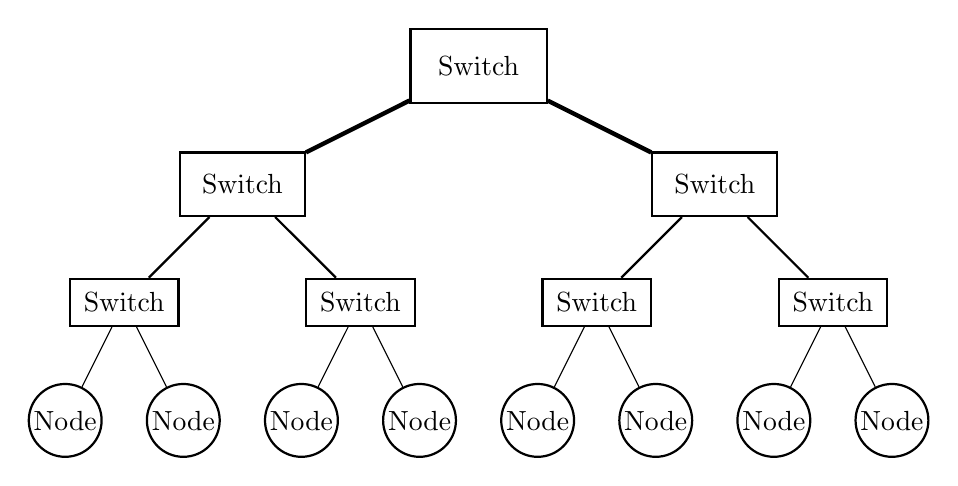
\begin{tikzpicture}[thick, node distance=1em]
	
	\begin{scope}[every node/.style={draw,rectangle,thick},inner sep=1.0em]
		\tikzstyle{level 1}=[sibling distance=6cm,every child/.style={ultra thick},inner sep=0.8em]
		\tikzstyle{level 2}=[sibling distance=3cm,every child/.style={thick},inner sep=0.5em]
		\tikzstyle{level 3}=[sibling distance=1.5cm,every child/.style={thin},inner sep=0.1em]
		
		\node {Switch}
			child {node {Switch}
				child {node {Switch}
					child {node [circle] {Node}}
					child {node [circle] {Node}}
				}
				child {node {Switch}
					child {node [circle] {Node}}
					child {node [circle] {Node}}
				}
			}
			child {node {Switch}
				child {node {Switch}
					child {node [circle] {Node}}
					child {node [circle] {Node}}
				}
				child {node {Switch}
					child {node [circle] {Node}}
					child {node [circle] {Node}}
				}
			}
		;
	\end{scope}
	
\end{tikzpicture}

						\caption{Basic fat tree links.}
						\label{fig:fat-tree-concept}
					\end{subfigure}
					
					\vspace{1em}
					
					\begin{subfigure}[t]{\textwidth}
						\center
						\input{figures/fat-tree-closs}
						\caption{Folded Clos network.}
						\label{fig:fat-tree-closs}
					\end{subfigure}
					
					\caption[Fat tree topologies.]{Fat tree topologies. Thicker lines
					represent higher bandwidth.}
					\label{fig:fat-tree}
				\end{figure}
			
			\subsubsection{Tori}
			
				The most common topology which features in all but one of the top-five
				is the torus (also known as a $k$-ary $n$-cube). In this topology, nodes
				are arranged in a $n$-dimensional mesh. Nodes at the extreme edges of
				the mesh are connected together to form a torus. In the 2D case this can
				be visualised as in figure \ref{fig:forming-a-torus}. Starting with a
				regular 2D mesh (figure \ref{fig:torus-flat}), the top- and bottom-most
				nodes are connected together to form a tube (figure
				\ref{fig:torus-pipe}).  Then the left- and right-most nodes of the tube
				are connected together forming a torus (figure \ref{fig:torus-3D}).
				Though harder to visualise, this process generalises to toruses of
				higher dimensions.
				
				Each node is able to communicate directly with its immediate neighbours
				in each dimension, that is above, below, left and right in the 2D case.
				More distant nodes are able to communicate by forwarding messages via
				intermediate nodes.
				
				Because nodes in a torus only communicate directly with their
				neighbours, the switches required in each node may be of a low radix
				compared to those in the fat tree. For an $n$-dimensional torus, each
				node requires a radix $n+1$ switches independent of the total number of
				nodes in the system.
				
				Compared with a fat tree, however, a greater number of hops is required
				in the worst case where two nodes are distant. In a torus $k$ nodes long
				in each of $n$ dimensions the worst case path length is $\frac{kn}{2}$
				\cite{dally04}. As a result, though the individual hops are less
				expensive, the time taken to broadcast a message to all nodes in a large
				Blue Gene/Q supercomputer such as Sequoia is 17.19$\mu$s compared to
				9$\mu$s for the same operation in Tianhe-2 \cite{morozov12}.
				
				Higher dimensional toruses are also easily partitioned into a number of
				lower-dimensional toruses or meshes to allow machines to be shared
				between many independent computing tasks \cite{yokokawa11,chen11}.
				
				\begin{figure}
					\begin{subfigure}[t]{\textwidth}
						\center
						\input{figures/torus-flat}
						\caption{Mesh (Grey lines show wrap-around connections added in a
						torus)}
						\label{fig:torus-flat}
					\end{subfigure}
					
					\vspace{1em}
					
					\begin{subfigure}[t]{\textwidth}
						\center
						\input{figures/torus-pipe}
						\caption{Rolled into a tube}
						\label{fig:torus-pipe}
					\end{subfigure}
					
					\vspace{1em}
					
					\begin{subfigure}[t]{\textwidth}
						\center
						\input{figures/torus-3D}
						\caption{Bent into a torus}
						\label{fig:torus-3D}
					\end{subfigure}
					
					\caption{Transformation of a mesh into a torus.}
					\label{fig:forming-a-torus}
				\end{figure}
		
		\subsection{Interconnect}
			
			%Many now using optical to transmit between cabinets. Electrical still
			%rules the waters for inter-card stuff.
			
			The physical links responsible for connecting machines together is another
			important factor in the performance achievable by a given interconnection
			system. The current state-of-the-art techniques fall into two categories:
			electrical (`high-speed serial') and optical transmission.
			
			Electrical transmission technologies are generally much cheaper than
			optical for short distances and lower bandwidths. As a result connections
			between physically neighbouring nodes are almost universally connected via
			such links. In systems such as Blue Gene/Q and Tianhe-2 optical links are
			used to connect between different cabinets in the system
			\cite{dongarra13,prickett10}. These optical links are able to carry the
			equivalent of many electrical signals over longer distances at the expense
			of more complex hardware requirements for transmitters and receivers.
			
			The topology of a network can greatly influence the difficulty of
			physically connecting nodes arranged in cabinets. The use of cabinets
			essentially map the physical nodes into an approximately 2D sheet. As a
			result, for torus networks of more than two dimensions, links which are
			physically short in higher dimensions can result in long wires between
			distant cabinets. For hierarchical networks such as fat trees, long wires
			can result from the need to connect together desperate parts of a system
			at the higher levels of the hierarchy. Long wires are both more complex to
			connect and require more expensive link technologies. The preliminary work
			described in \S\ref{sec:wiring-up-large-spinnaker-machines} explores these
			issues in further detail.
			
			% TODO: What am I trying to say here?
			
			% At a very high level, these two systems operate in a similar fashion.
			% Messages are broken down into individual bits by a transmitter and then
			% sent one bit at a time across a pair of wires or a glass fibre for
			% high-speed serial and optical transmission respectively. At the receiver
			% the bits are reassembled into a complete message.
	
	\section{Hardware Neural Simulators}
		
		% Discuss various neural-simulation based approaches, e.g. neuromorphic
		% computers, Blue Brain, BrainScaleS, FPGA based things, speak to Franchesco.
		
		Current super computers are heavily focused on computation-heavy tasks as is
		apparent from the use of of hundreds of thousands of high-end processor
		cores in the Top500's top five machines. Projects such as the Blue Brain
		project \cite{markram06} are able to make use of such computationally
		powerful machines in the simulation of relatively small ANNs of tens of
		thousands of biologically realistic neurons. Large ANN using the less
		realistic models of neuron behaviour change the balance between computation
		and communication. Requiring relatively little computation for each neuron
		but instead require vast amounts of communication, conventional super
		computers are a poor fit and, as a result, alternative architectures have
		been developed for neural simulation.
		
		There are three distinct approaches being taken to designing hardware for
		neural simulation. One is to use analog electronic components for the
		entire system, another is to mix analog and digital components and a final
		approach is to use traditional digital components. These three approaches
		and their merits are described below.
		
		\subsection{Analog}
		
			Though analog technology has long been out of favour for general purpose
			computing, it has been suggested for the purpose of neural simulation as
			it is ultimately designed to model an analog system: the brain. Neural
			models are highly fault-tolerant and does not rely on the assumption that
			values will be calculated or communicated precisely. Modern digital
			computers, by contrast, have rigid requirements for the precision of
			values and so dedicate vast amounts of hardware and energy to guaranteeing
			such unneccessary precision making analog simulators an attractive
			approach.
			
			A wide range of techniques for implementing the required functions in
			analog circuitry have been proposed
			\cite{graf86,holler89,agranat90,azghadi13}.  The analog circuits are often
			very simple and require far less power than the equivalent calculations
			running on a general purpose processor \cite{misra10}. Even though the
			lack of precision yielded by analog circuits is not a problem for neural
			simulation, the lack of consistency is. The same analog circuit may have
			widely different characteristics in one part of the chip compared to
			another due to variations in the silicon wafer. In addition circuits must
			tolerate changes in temperature and voltage, a task which is substantially
			more challenging for analog circuits compared to their digital
			counterparts. Finally, these systems make assumptions about the type of
			neural models that will be simulated limiting them to simulating only a
			handful of similar models. As a result, the current generation of analog
			simulators lag behind the state-of-the-art in terms of ease-of-use and
			flexibility.
		
		\subsection{Mixed Mode}
			
			So-called `mixed mode' systems have been designed such as
			\cite{heittmann02} which combines analog computational components with
			digital memory yielding systems with efficient computation and dense
			storage. In \cite{murray91} another mixed mode system is given which again
			features analog computation of neuron behaviour but uses digital signals
			to distribute spike transmission allowing easier and more flexible routing.
			
			While offering improvements over purely analog systems, many of the same
			drawbacks with variability and flexibility still apply.
		
		\subsection{Digital}
			
			Various groups have developed custom, digital, on-chip neural simulators
			\cite{prange93,jahnke96,schoenauer99,mehrtash03}. While successful in
			allowing relatively large numbers of neurons to be simulated, around 1
			million in the case of \cite{mehrtash03}, along with the analog and mixed
			mode designs above, these approaches are fundamentally restricted to only
			the models the designers originally intended. This lack of flexibility
			along with the increasing costs of designing custom silicon has pushed
			researchers away from this approach.
			
			FPGAs (field programmable gate arrays) are, essentially, chips which can
			be electrically reprogrammed with custom logic circuits. They are now
			widely used in place of custom chips for performance-sensitive, highly
			specialised tasks as well as prototyping and development of conventional
			chips. Work using FPGAs to simulate neural models such as
			\cite{hellmich05} have allowed around half a million neurons with
			realistic numbers of connections between them to be simulated. Despite
			being considerably cheaper and far more flexible than completely custom
			hardware, FPGA development is still much slower than developing for
			general purpose CPUs and so still yields relatively inflexible systems.
			
			Finally, architectures based on general purpose digital processors are
			able to provide a great degree of flexibility at the expense of greater
			overhead\cite{furber07}. The SpiNNaker project, described in detail in the
			next section, has developed an architecture which combines many low-power
			processors which run neural simulations in software.
	
	
	\section{SpiNNaker}
		
		\label{sec:spinnaker}
		
		% The architecture focused on by my research.
		
		The SpiNNaker project is developing a super computer architecture designed
		for running real-time simulations of large networks of SNNs. In particular,
		its designed to be very flexible making as few assumptions about the
		function of individual neurons as possible\cite{furber06}.
		
		To achieve this flexibility SpiNNaker will combine over one million
		energy-efficient, general purpose, mobile phone grade CPUs with a custom
		interconnect network designed to tackle the communication bound problem of
		simulating large networks of simple neurons. The machine is planned to
		support networks of around one billion ($10^9$) spiking neurons (around 1\%
		of a human brain) in biological real-time.
		
		Due to the machine's flexibility and novel interconnect it presents many
		opportunities for experimentation and so has been the focus of much of the
		preliminary work done so far. The rest of this section describes SpiNNaker
		highlighting areas relevant to the preliminary work and final project.
		
		\subsection{Architecture}
			
			% Due to the neural networks we're using, this is the sort of topology that
			% was made. Good for sending short messages to many targets at once. Bad at
			% system stuff though, also currently very much 2D unlike the brain. Have a
			% hexagonal toroid (picture) which is nice and regular but a pain to wire up.
			
			SpiNNaker is made up of a 2D toroid\footnote{A toroid, in this context, is
			the generalisation of a torus where nodes are connected to more than $2n$
			neighbours where $n$ is the number of dimensions.} of chips where each
			chip connects to its six neighbouring chips as shown in figure
			\ref{fig:spinnaker-chips}. The system can be flexibly extended by simply
			enlarging the toroid and adding more chips. The size of the network is
			only limited by the size of address fields used to route spikes around the
			system.
			
			Each SpiNNaker chip contains 18 low-power ARM processor cores connected
			together via a network on chip (NoC) as shown in figure
			\ref{fig:spinnaker-chip}. Each core has a small amount of private memory
			and has access to a larger, chip-wide memory (not shown). Finally the chip
			contains a router responsible for sending and receiving messages from the
			six neighbouring chips as well as forwarding on messages destined for
			another chip.
			
			% TODO: Fix this figure as the CPUs don't really go through the NoC to the
			% router for normal use...
			
			\begin{figure}
				\center
				\begin{subfigure}[b]{0.49\textwidth}
					\center
					\input{figures/spinnaker-chip}
					\caption{SpiNNaker chip\\\color{white}.}
					\label{fig:spinnaker-chip}
				\end{subfigure}
				\begin{subfigure}[b]{0.49\textwidth}
					\center
					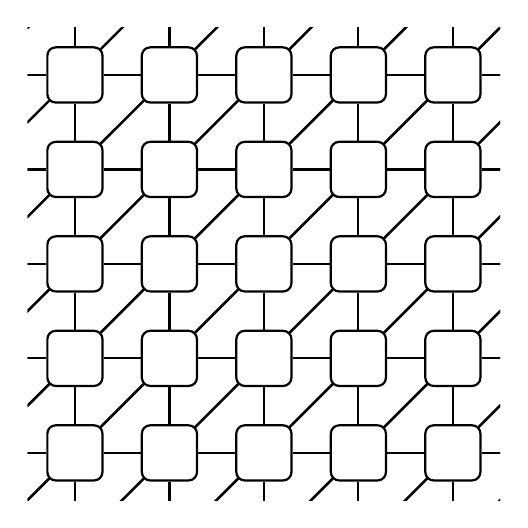
\begin{tikzpicture}[thick]
	
	\def\width{5}
	\def\height{5}
	
	% Space between node centers
	\def\spacescale{1.2}
	
	% Rounding on edges of chips
	\def\rounding{0.7ex}
	
	\pgfmathtruncatemacro{\widthh}{\width-1}
	\pgfmathtruncatemacro{\heightt}{\height-1}
	
	\tikzset{
		chip/.style={draw,rounded corners=\rounding,minimum size=0.7cm}
	}
	
	% Clip off the extra row of chips around the edge that are added to ensure we
	% end up with lots of wires dangling off the edge.
	\clip (-0.5*\spacescale,-0.5*\spacescale) rectangle
	      (\spacescale*\width-0.5*\spacescale,
	       \spacescale*\height-0.5*\spacescale);
	
	% The chips
	\foreach \x in {-1,...,\width}{
		\foreach \y in {-1,...,\height}{
			\node [chip] (chip X\x Y\y) at (\spacescale*\x, \spacescale*\y) {};
		}
	}
	
	% Edge links...
	\tikzset{
		edge wire/.style={}
	}
	
	% The wires
	\foreach \x in {0,...,\width}{
		\foreach \y in {0,...,\height}{
			\pgfmathtruncatemacro{\xx}{\x-1}
			\pgfmathtruncatemacro{\yy}{\y-1}
			
			% South-West to North-East
			\ifthenelse{\xx < 0 \OR \xx = \widthh \OR \yy < 0 \OR \yy = \heightt}{
				\draw [shorten >=-0.5*\rounding,shorten <=-0.5*\rounding]
				      [edge wire]
				      (chip X\x Y\y) to (chip X\xx Y\yy);
			}{
				\draw [shorten >=-0.5*\rounding,shorten <=-0.5*\rounding]
				      (chip X\x Y\y) to (chip X\xx Y\yy);
			}
				
				% South to North
			\ifthenelse{\yy < 0 \OR \yy = \heightt}{
				\draw [edge wire]
				      (chip X\x Y\y) to (chip X\x Y\yy);
			}{
				\draw (chip X\x Y\y) to (chip X\x Y\yy);
			}
				
				% West to East
			\ifthenelse{\xx < 0 \OR \xx = \widthh}{
				\draw [edge wire]
				      (chip X\x Y\y) to (chip X\xx Y\y);
			}{
				\draw (chip X\x Y\y) to (chip X\xx Y\y);
			}
		}
	}
	
\end{tikzpicture}

					\caption{Connections between chips (dots) with wrap-around
					connections not shown}
					\label{fig:spinnaker-chips}
				\end{subfigure}
				
				\caption{Overview of the SpiNNaker architecture.}
				\label{fig:spinnaker-architecture}
			\end{figure}
		
		\subsection{Routing}
			
			% Routing is done by table based router. Entries for each turn or fork in a
			% packet path. Limited number of entries. Source address based routing (TLA
			% to be requested). All routing (currently) static and offline.
			
			The on-chip router is table based meaning that routing decisions are taken
			based on a set of pre-determined choices loaded into a memory before
			simulations begin. The router operates on individual packets of data which
			are either 40 or 72 bits in length. These packets are very short compared
			to the type of interconnection network commonly used in super computers.
			Such networks are typically designed to transfer larger blocks of data,
			possibly many kilobytes long. SpiNNaker, however, is designed to primarily
			deal with SNNs where only the spikes' existence needs to be transmitted
			requiring little or no associated data.  The system supports four
			different kinds of packet:
			
			\begin{description}
				
				\item[Point-to-Point (P2P)] Addressed to an individual chip and will be
				passed to the core arbitrarily selected by the chip as the `monitor'
				core. Packets are routed using a routing table.
				
				\item[Multicast (MC)] Sent by a single core and delivered to a
				predetermined set of cores in the system. Packets are routed according
				to their source address and do not explicitly store the destination
				cores. Packets are routed using a routing table.
				
				\item[Fixed Route (FR)] Automatically routed to a predefined central
				point in the system. Used, for example, to collect diagnostic
				information back to the host machine. By not requiring an address a
				larger payload can be attached.
				
				\item[Nearest Neighbour (NN)] Routed to the immediate neighbours of a
				chip without the need for a routing table. On system start up routing
				tables have not been initialised and so NN packets are used to initially
				load the tables.
				
			\end{description}
			
			\subsubsection{Routing Scheme}
				
				% Current routing is very naive dimension order routing. Also highly
				% static and doesn't respond to network utilisation. The internet is
				% dynamic, maybe this should be too?
				
				Table based routing allows a wide array of possible routing schemes to
				be implemented conditional to two key constraints. First, the route
				taken by a packet with a particular source/destination address will
				always take the same path through the system. This is known as
				deterministic oblivious routing as the scheme is unaware of the system's
				state and cannot react to load imbalance. It is worth noting that
				schemes still exist which can improve load balance in the general case
				\cite{singh02}.
				
				\begin{figure}
					\center
					\input{figures/dimension-order-routing}
					\caption[Dimension order routing in SpiNNaker.]{Dimension order routing
					in SpiNNaker showing a path from node $S$ to node $T$.}
					\label{fig:dimension-order-routing}
				\end{figure}
				
				Current versions of the routing software uses simple dimension order
				routing. Here, the three axes along which packets can travel are
				considered to be three `dimensions'\footnote{The three dimensions in
				SpiNNaker's toroid are not orthogonal as would be the case in a
				conventional torus network. This is the cause of some of the slightly
				unintuitive properties of the topology.}. Packets travel along a given
				dimension until they can get no closer at which point they move onto the
				next dimension as shown in figure \ref{fig:dimension-order-routing}.
				Such paths are easily computed as shown in \cite{nocetti02} and are
				minimal in the number of hops required.
			
			\subsubsection{Multicast}
				
				% Not much stuff on this at the moment. I am so shit I've not read
				% anything about it anyway so that needs to change.
				
				Multicast packets allow SpiNNaker to efficiently handle the distribution
				of spikes from heavily connected neurons in the system without requiring a
				unique packet to be sent to each destination. Instead a
				single packet is transmitted which is able to `fork' in order to reach
				multiple processors later in its journey.
				
				Unlike P2P packets, for which the route for every possible chip address
				(16 bits) can be stored in a routing table of around 25 kilobytes, MC
				packets are routed based on a 32 bit key which uniquely identifies the
				neuron which fired.  Exhaustively storing the route for every possible
				32-bit key is not possible since 24 bits are required for each
				entry\footnote{One bit for each of the 18 cores and 6 external links
				specifying if the packet should be routed to that output} thus requiring
				a 12 gigabyte routing table.
				
				Instead of an exhaustive table, one with 1,024 entries is used. The
				router looks up the 32-bit key of MC packets and, if a matching entry
				exists, uses that entry to decide where to route the packet. If no entry
				exists, the packet is forwarded to the link physically opposite the one
				through which it entered. As a result, the routing table only requires
				an entry when the packet changes direction or is to be delivered to a
				core.
				
				Since the route for messages with a given key will only pass through or
				change direction in a very small number of places, most routers in the
				system won't need to include an entry in their routing table. As a
				result this small size of routing table is adequate.
				
				\begin{figure}
					\begin{subfigure}[b]{0.24\textwidth}
						\center
						\input{figures/multicast-routing-a}
						\caption{}
						\label{fig:multicast-routing-a}
					\end{subfigure}
					\begin{subfigure}[b]{0.24\textwidth}
						\center
						\input{figures/multicast-routing-b}
						\caption{}
						\label{fig:multicast-routing-b}
					\end{subfigure}
					\begin{subfigure}[b]{0.24\textwidth}
						\center
						\input{figures/multicast-routing-c}
						\caption{}
						\label{fig:multicast-routing-c}
					\end{subfigure}
					\begin{subfigure}[b]{0.24\textwidth}
						\center
						\input{figures/multicast-routing-d}
						\caption{}
						\label{fig:multicast-routing-d}
					\end{subfigure}
					\caption[Multicast routing examples.]{Multicast routing examples from
					$S$ to $T_1$ and $T_2$.}
					\label{fig:multicast-routing}
				\end{figure}
				
				In multicast routing, the choice of where a route should fork can have a
				great impact on both system load, packet latency and routing table entry
				usage. Figure \ref{fig:multicast-routing} shows several examples of
				valid multicast routings which fork at different points, each with
				differing trade-offs. For example, figures (b) - (d) are all optimal in the total
				number of `hops' required while (a), (c) and (d) are optimal in the
				number of routing entries required.
				
				As well as guaranteeing short paths and that no routing table requires
				more than 1,024 entries, the multicast routing scheme chosen must
				attempt to ensure an even load-balance by avoiding over-using certain
				links. Various heuristic approaches based on extensions to Lee's
				algorithm have been proposed for future versions of the routing
				software\cite{davidson13}.
			
			\subsubsection{Emergency Routing}
				
				If a packet's intended route is blocked, for example due to a broken
				link, `emergency routing' via an adjacent chip can optionally be
				attempted as shown in figure \ref{fig:emergency-routing}. This novel
				approach allows the system to automatically recover from certain link
				failures without immediate manual intervention. This mechanism has been
				shown to improve the system's fault tolerance \cite{navaridas09}.
				
				\begin{figure}
					\center
					\begin{tikzpicture}[inner sep=0]
	
	\clip (2cm,1.25cm) rectangle +(3cm,3.5cm);
	
	\begin{scope}[hexagonXYZ,minimum size=0.25cm,inner sep=0]
		\foreach \y in {1,...,8}{
			\foreach \x in {1,...,16}{
				\node (chip \x \y) at (\x,\y) [fill,circle] {};
			}
		}
	\end{scope}
	
	\begin{scope}
		\foreach \y in {2,...,7}{
			\foreach \x in {2,...,15}{
				\pgfmathtruncatemacro{\xx}{\x+1}
				\pgfmathtruncatemacro{\yy}{\y+1}
				\draw (chip \x \y) -- (chip \xx \yy);
				
				\pgfmathtruncatemacro{\xx}{\x-1}
				\pgfmathtruncatemacro{\yy}{\y-1}
				\draw (chip \x \y) -- (chip \xx \yy);
				
				\pgfmathtruncatemacro{\xx}{\x+1}
				\pgfmathtruncatemacro{\yy}{\y+0}
				\draw (chip \x \y) -- (chip \xx \yy);
				
				\pgfmathtruncatemacro{\xx}{\x-1}
				\pgfmathtruncatemacro{\yy}{\y+0}
				\draw (chip \x \y) -- (chip \xx \yy);
				
				\pgfmathtruncatemacro{\xx}{\x+0}
				\pgfmathtruncatemacro{\yy}{\y+1}
				\draw (chip \x \y) -- (chip \xx \yy);
				
				\pgfmathtruncatemacro{\xx}{\x+0}
				\pgfmathtruncatemacro{\yy}{\y-1}
				\draw (chip \x \y) -- (chip \xx \yy);
			}
		}
	\end{scope}
	
	\node [below right=0.5ex of chip 53] {\contour{white}{$S$}};
	\node [below right=0.5ex of chip 64] {\contour{white}{$T$}};
	
	\draw [white,ultra thick=3pt] (chip 53) -- (chip 64);
	\draw [style=help lines] (chip 53) -- coordinate (badlink) (chip 64);
	
	\draw [red,thick]
	      ([shift={(-0.7ex,-0.7ex)}]badlink)
	   -- ([shift={(+0.7ex,+0.7ex)}]badlink)
	      ([shift={(-0.7ex,+0.7ex)}]badlink)
	   -- ([shift={(+0.7ex,-0.7ex)}]badlink);
	
	\draw [black,line width=3pt] (chip 53.center) -- (chip 54.center);
	\draw [black,line width=3pt] (chip 54.center) -- (chip 64.center);
	
\end{tikzpicture}


					\caption[Emergency routing example.]{Emergency route from $S$ to $T$
					when the normal route is unavailable.}
					\label{fig:emergency-routing}
				\end{figure}
			
		
		\subsection{Hardware Abstractions}
			
			% SpiNNaker is made up of 18 core chips on 48-chip boards in 12 card racks
			% in 5-rack cabinets in a 10 cabinet system. Woah.
			
			The largest SpiNNaker system will contain 1,036,800 cores spread over
			57,600 chips.  These chips are split up into 1,200 circuit boards of 48
			chips each as shown in figure \ref{fig:spinn4labelled}.
			
			\begin{figure}
				\center
				\begin{tikzpicture}[thick]
	
	\node[anchor=south west,inner sep=0] at (0,0) (image)
		{\includegraphics[width=0.5\textwidth]{figures/spinn4.png}};
	
	\begin{scope}[x={(image.south east)},y={(image.north west)}]
		%% Help with drawing
		%\draw[help lines,xstep=.1,ystep=.1] (0,0) grid (1,1);
		%\foreach \x in {0,1,...,9} { \node [anchor=north] at (\x/10,0) {0.\x}; }
		%\foreach \y in {0,1,...,9} { \node [anchor=east] at (0,\y/10) {0.\y}; }
		
		\draw [decorate,decoration={brace,raise=1ex,amplitude=1ex}]
		      (0.02,0.5) -- coordinate (left-label) (0.02,1.0);
		\node [left=1em of left-label,text width=3.5cm,align=center]
		      {High-Speed Links\\(Board-to-Board)};
		
		\draw [decorate,decoration={brace,raise=1ex,amplitude=1ex}]
		      (0.97,1.0) -- coordinate (right-label) (0.97,0.5);
		\node [right=1em of right-label,text width=3.5cm,align=center]
		      {High-Speed Links\\(Other I/O)};
		
		\draw [decorate,decoration={brace,raise=1ex,amplitude=1ex}]
		      (1.0,0.23) -- coordinate (power-label) (1.0,0.02);
		\node [right=1em of power-label] {Power Connector};
		
		\draw [decorate,decoration={brace,raise=1ex,amplitude=1ex}]
		      (0.0,0.08) -- coordinate (eth-label) (0.0,0.22);
		\node [left=1em of eth-label] {Ethernet};
	\end{scope}
	
\end{tikzpicture}

				\caption{48-chip SpiNNaker circuit board.}
				\label{fig:spinn4labelled}
			\end{figure}
			
			Each board is equipped with a number of high-speed links, six of which are
			used to connect the board's chips them to their neighbours on other
			boards. The other six links are reserved for connecting other I/O such as
			sensors, such as the silicon retina, and robotic platforms
			\cite{davies10}. An Ethernet connection is also present to provide a
			simple, low-bandwidth link to an external host system.
			
			\begin{figure}
				\center
				\includegraphics[width=0.5\textwidth]{figures/spiNNaker103.jpg}
				\caption{Partially populated rack of SpiNNaker boards.}
				\label{fig:spiNNaker103}
			\end{figure}
			
			Groups of twenty-four boards are then placed in racks such as in figure
			\ref{fig:spiNNaker103} which are in turn placed, five-high, into ten
			cabinets to complete the largest planned machine. Further details of this
			arrangement are given later in
			\S\ref{sec:wiring-up-large-spinnaker-machines} where preliminary work on
			wiring schemes for the machine is described.
		
		\subsection{Connecting Boards Together}
			
			% Describe what the edge links have.  Boards are connected together via high
			% speed serial links. 8 links per board. First gen had two spare
			% connections, new one has ring and one spare. What can the spares be used
			% for?
			
			% TODO: Reword
			The chips on each circuit board are logically laid out as shown in figure
			\ref{fig:chipsOnBoard}. Touching edges represent a chip-to-chip connection
			which uses a delay insensitive, parallel `2-of-7' communications scheme
			similar to that used in the on-chip network requiring 16 wires per link.
			If this technology was used to connect boards together 768 wires would be
			required.  This would be prohibitively expensive requiring expensive,
			highly specialised cables and connectors. Instead, an alternative
			technology, known as high-speed serial, is used which replaces the 768
			wires with only 24 which can be carried by cheap commodity cables. This
			technology allows eight chip-to-chip connections to share a single cable
			grouped as shown in the figure.
			
			\begin{figure}
				\center
				\input{figures/chipsOnBoard}
				\caption{Logical arrangement of chips on a circuit board.}
				\label{fig:chipsOnBoard}
			\end{figure}
			
			In order to construct a toroid, at least three boards must be combined as
			shown in figure \ref{fig:threeboard} (an arrangement known as a
			threeboard).  Figure \ref{fig:threeboardSliced} shows how the threeboard
			arrangement can be turned into a sheet which in turn can be turned into a
			toroid as shown earlier in figure \ref{fig:forming-a-torus}.
			
			\begin{figure}
				\begin{subfigure}[b]{0.45\textwidth}
					\center
					\input{figures/threeboard}
					\caption{Threeboard}
					\label{fig:threeboard}
				\end{subfigure}
				\begin{subfigure}[b]{0.45\textwidth}
					\center
					\input{figures/threeboardSliced}
					\caption{Sliced into a sheet}
					\label{fig:threeboardSliced}
				\end{subfigure}
				
				\caption[A `threeboard'.]{A `threeboard', the minimal configuration of
				boards yielding a toroid.}
			\end{figure}
			
			Arbitrarily large systems can be produced by repeating the threeboard
			pattern to create larger toroids.
	
	\section{High-Speed Serial}
		
		\label{sec:high-speed-serial}
		
		% Always on, power hungry. Better to have few of these running fast rather
		% than many running slow? Where are these used. What do they replace.
		
		High-speed serial is the general name for a technology which allows
		high-bandwidth links to be constructed using very few electrical wires.
		These links are the basis of many widely used technologies ranging from
		S-ATA, used for attaching consumer-grade hard disks to computers
		\cite{sataio}, to the InfiniBand interconnect designed for super computers
		\cite{infinibandta}.
		
		Compared to older technologies such as simple parallel buses, high-speed
		serial links require more complex hardware to implement and so tend to be
		reserved for chip-to-chip or board-to-board connections. Indeed, they are
		the basis of many current Top500 super computer interconnects as well as
		SpiNNaker's board-to-board links. This section outlines the basics of the
		technology and the reasons for its increased complexity.
		
		\subsection{From Parallel to Serial}
			
			Traditionally, signals between components in a system have been carried by
			a set of parallel wires. Each wire carried a single bit allowing multiple
			bits to be transmitted at once. Figure \ref{fig:parallel-example-no-skew}
			shows eight parallel signals being used to transmit a message. The
			electrical signal being sent down each wire is sampled at the tick of a
			clock (the vertical lines in the figure) and the eight bits are
			interpreted as an ASCII character.
			
			In practice each of the wires carrying the parallel signal will have
			slightly differing electrical properties due to imperfections during
			manufacturing such as slightly differing lengths. These differences result
			in the signals taking different amounts of time to travel along the wires,
			an effect known as skew. For a long time the skew remained insignificant
			compared to the time between samples being taken of the parallel signal.
			As clock speeds increased, however, skew started to become significant
			enough to cause some of the parallel signals to arrive so far apart
			relative to the clock that some would be incorrectly sampled by the
			receiver resulting in transmission errors such as in figure
			\ref{fig:parallel-example-skew}.
			
			\begin{figure}
				\begin{subfigure}[b]{0.49\textwidth}
					\center
					\input{|"python figures/parallel_comms.py 'Hello, World!' 1.0 1.3 0"}
					\caption{No skew}
					\label{fig:parallel-example-no-skew}
				\end{subfigure}
				\begin{subfigure}[b]{0.49\textwidth}
					\center
					\input{|"python figures/parallel_comms.py 'Hello, World!' 1.0 1.3 0.7"}
					\caption{With skew}
					\label{fig:parallel-example-skew}
				\end{subfigure}
				
				\caption{Parallel signalling example.}
				\label{fig:parallel-example}
			\end{figure}
			
			Unfortunately, since wiring technology has been unable to improve fast
			enough to keep skew acceptably small for all but the shortest connections,
			parallel signalling has been replaced with high-speed serial signalling.
			Here, bits are sent one after another as shown in figure
			\ref{fig:serial-example}. Because there is only one signal, the problem of
			skew is eliminated.
			
			\begin{figure}
				\center
				\begin{tikzpicture}
					\input{|"python figures/serial_comms.py '' 'Hello, World!' 1 0 0 0 0 0.4 0.2"}
				\end{tikzpicture}
				
				\caption{Serial signalling example.}
				\label{fig:serial-example}
			\end{figure}
		
		
		\subsection{Clock Recovery}
			
			In systems using parallel links it is often possible for the two devices
			to share a common clock in order for the receiver to be able to determine
			the correct time to sample the incoming signal. In high-speed serial
			systems the possible skew between the data signals and an associated clock
			signal would be unacceptable. As a result, the receiver must determine the
			exact clock frequency and phase by observing the incoming data signal.
			
			A phase locked loop (PLL) is a device which is able to synthesize the
			original clock signal given a stream of data which changes sufficiently
			often \cite{athavale05}. In order to be effective, the incoming data
			stream must transition between 0 and 1 sufficiently frequently for the PLL
			to be able to `lock on'. For example it is not possible to infer the clock
			from long string of 0s.
			
			Unfortunately real data can legally contain such long strings of the same
			value. Figure \ref{fig:8b10b-example} shows a string which contains some
			ASCII characters followed by a sequence of zeros which could cause a PLL
			to lose its lock on the clock signal. To work around this, the raw data is
			encoded using 8b/10b coding \cite{widmer83}\footnote{8b/10b is being
			replaced by alternatives such as 64b/66b. These are more complex but
			suffer less overhead while offering essentially the same advantages as
			8b/10b.}. Data is encoded in blocks of 8 bits into 10 bit symbols as shown
			in the figure.  This encoding adds an additional 20\% of overhead but
			grantees that no long sequences of 0 or 1 will be present in the output.
			
			\begin{figure}
				\center
				\begin{tikzpicture}
					\input{|"python figures/serial_comms.py 'Raw' 'Zero*****' 1 0 0 0 0 0.4 0.2"}
					\begin{scope}[yshift=-1.5cm]
						\input{|"python figures/serial_comms.py '8b/10b' 'Zero*****' 1 0 0 0 1 0.4 0.2"}
					\end{scope}
				\end{tikzpicture}
				
				\caption{8b/10b encoding example.}
				\label{fig:8b10b-example}
			\end{figure}
		
		
		\subsection{Electrical Considerations}
			
			Typically, data is transmitted down a wire by varying the voltage applied
			to it by the transmitter, for example 5 volts may indicate a binary `1'
			and 0 volts a binary `0'. Unfortunately, the voltage assumed to be 0 volts
			by two connected systems may not be exactly equal in practice (a
			phenomenon known as voltage imbalance). Directly connecting these
			imbalanced systems would cause a current to flow between them which wastes
			energy and may damage the system. To resolve this the two systems may be
			connected via a capacitor which allows \emph{changes} in voltage to
			propagate between the two systems while the actual voltage does not.
			
			With the introduction of a capacitor into the link, a new problem emerges.
			If, over time, more `1's are transmitted than `0's the capacitor can
			charge up gradually causing the receiver to falsely detect a `0'. The
			8b/10b code, described previously, also has the property that the number
			of `1's and `0's remains equal over time which eliminates this effect.
			This is known as maintaining DC balance. This can be seen in figure
			\ref{fig:8b10b-example} where the symbol for \texttt{0x00}, labelled
			\texttt{D.00.0}, alternates between two values to maintain the balance of
			`0's and `1's transmitted.
			
			Electrical wires are also subject to external noise which can cause the
			value of a bit to be misread. To alleviate this, the signal is transmitted
			twice with one wire carrying the signal and the other its negation. If
			these wires are kept physically close they are likely to experience
			exactly the same pattern of noise as shown in figure
			\ref{fig:differential-encoding}. The receiver takes the difference of the
			two signals which causes the noise, which is equal in both, to be
			cancelled out leaving the original data intact.
			
			\begin{figure}
				\center
				\begin{tikzpicture}
	\input{|"python figures/serial_comms.py 'Noise' 'Hello, World!' 0 0.2 1 0 0 0.38 0.2"}
	
	\begin{scope}[yshift=-1.0cm]
		\input{|"python figures/serial_comms.py 'Signal+' 'Hello, World!' 0 0.2 0 0 0 0.38 0.2"}
	\end{scope}
	
	\begin{scope}[yshift=-2.0cm]
		\input{|"python figures/serial_comms.py 'Signal-' 'Hello, World!' 0 0.2 0 1 0 0.38 0.2"}
	\end{scope}
	
	\begin{scope}[yshift=-3.0cm]
		\input{|"python figures/serial_comms.py 'Difference' 'Hello, World!' 1 0.0 0 0 0 0.38 0.2"}
	\end{scope}
	
\end{tikzpicture}


				
				\caption{Eliminating noise using differential coding.}
				\label{fig:differential-encoding}
			\end{figure}

	\chapter{Preliminary Work}
	
	\section{High-Speed Serial Link Modelling}
		
		In order to understand the effects of inserting non-uniformity to the
		SpiNNaker Interconnect caused by the high speed links.
		
		\subsection{Objectives}
			Try and find out what is going on.
		
		\subsection{Results}
			Found a significant increase in average latency. Maybe this could be
			overcome by making more use of that added processing time by jumping on
			further ahead? Further simulation needs to be done anyhow...
	
	\section{SpiNNaker PCI-Express Interface}
		
		One way of getting data from one part of the machine to the other would be
		not to just dump it through another link but to pull it straight out into a
		conventional computer via PCI-Express and then maybe re-route it with
		fancier software or via the web.
		
		\subsection{PCI-Express}
			
			What is PCI-Express? How does it work? Where is it found?
		
		\subsection{High Speed Serial on FPGA}
			
			What is an FPGA? We have one on the boards. FPGAs contain hard-wired
			blocks which do special purpose things, one such job is to do PCI-Express.
	
	\section{Wiring-Up Super Computers}
		
		A practical constraint on any interconnect is that it should be possible to
		wire it up. In particular constraints exist on both on wire length and the
		practical difficulty of connecting up the wires into the correct places.
		Computers usually placed in racks. Tool can be used to study wiring
		constraints of new links.
		
		\subsection{Wire-Length Limits}
			
			What type of signalling is possible? Why are long wires bad? How long is
			long? Why not just the average wire length?
		
		\subsection{Topology}
			
			SpiNNaker has three dimensions of wiring connected in a torus. This has
			long wires. A torus intuitively has long wires along the way which causes
			a bit of a headache. You can slice it to make it rectangular, you can fold
			it to make the wires short (must fold 4x2) and divvy up into cabinets..
		
		\subsection{\emph{SpiNNer} Wiring Guide Generator}
			
			A tool was built, manipulates nodes which are pre-connected with the
			correct wiring graph. Produces instructions.
		
		\subsection{Further Work}
			
			Simplify instructions, alternative wirings.
	
	\section{Small-World Super Computers}
		
		In the same way that random search is generic (no free lunch), I tried
		adding random wires. This is backed up by Watts and Strogatz's small-world
		network producing algorithm. Built a model. Took into account wiring using
		techniques in Wiring-Up Super Computers.
		
		\subsection{Results}
			
			Even with wire-length limits in place, when folded the effect is still
			noticeable.
		
		\subsection{Further Work}
			
			Must try this with SpiNNaker topology and racks (maybe even better). Would
			like to formalise the result into a formula.
	
	\section{Place and Route}
		
		Tests written for the Place and Route system for SpiNNaker-103. Gained some
		experience with the task. 
		
		\subsection{Potential Improvements}
			
			The algorithms used for placement and routing are naive: generally greedy
			algorithms.




	\chapter{Research Plan}

	\section{Short Term}
		
		\subsection{SpiNNaker Interconnect Model}
		
			\subsubsection{Performance Benchmarking}
			
			\subsubsection{Interconnect Experiments}
		
		\subsection{Effects of Multicast}
		
		\subsection{Routing in Hybrid Topologies}
	
	\section{Longer Term}
		
		\subsection{Further Network Topologies}
		
		\subsection{`SpiNNaker 2' Architecture}
			
			\subsubsection{Types of Transmission}
			
			\subsubsection{Multiple Networks}


	\chapter{Conclusion}
	
	Parallel computing is big but tough. Interconnect in particular is a bit fun,
	especially for brain simulators.
	
	Current work has a rich selection of networks in use but for brain
	simulation??? In particular multicast seems a little less well trodden.
	
	My work looks at SpiNNaker and I have been working on simulating this and the
	problems relating for wiring etc.

	
\end{document}
